\documentclass[10pt,twocolumn,letterpaper]{article}

\usepackage{cvpr}
\usepackage{times}
\usepackage{epsfig}
\usepackage{graphicx}
\usepackage{amsmath}
\usepackage{amssymb}

% Include other packages here, before hyperref.

% If you comment hyperref and then uncomment it, you should delete
% egpaper.aux before re-running latex.  (Or just hit 'q' on the first latex
% run, let it finish, and you should be clear).
\usepackage[pagebackref=true,breaklinks=true,letterpaper=true,colorlinks,bookmarks=false]{hyperref}


\cvprfinalcopy % *** Uncomment this line for the final submission

\def\cvprPaperID{****} % *** Enter the CVPR Paper ID here
\def\httilde{\mbox{\tt\raisebox{-.5ex}{\symbol{126}}}}

% Pages are numbered in submission mode, and unnumbered in camera-ready
\ifcvprfinal\pagestyle{empty}\fi
\begin{document}

%%%%%%%%% TITLE
\title{Hammer of Dawn: An Automated Laser-Guided Turret}

\author{Nick Childers, Sean Ford, Marcus Jang\\
Unversity of California Santa Barbara\\
{\tt\small nickchilders@umail.ucsb.edu, sford@umail.ucsb.edu, marcusjang@gmail.com}
% For a paper whose authors are all at the same institution,
% omit the following lines up until the closing ``}''.
% Additional authors and addresses can be added with ``\and'',
% just like the second author.
% To save space, use either the email address or home page, not both
%\and
%Second Author\\
%Institution2\\
%First line of institution2 address\\
%{\small\url{http://www.author.org/~second}}
}

\maketitle
\thispagestyle{empty}

%%%%%%%%% ABSTRACT
\begin{abstract}
Our project is a laser guided turret. The turret consists of an Airsoft gun with a camera attached to it and will be able to freely rotate. The camera is used to find a laser point in its view and then point the turret at it. Next, a secondary laser that is attached to the turret will then be used to determine distance between the turret and the object it is pointing at. Once distance is known, adjustments can then be made to accurately shoot the Airsoft gun.
\end{abstract}

%%%%%%%%% BODY TEXT

\section{Introduction}


\section{Approach}


\subsection{Laser Identification}

Laser points have a very characteristic look to them. They tend to be small brightly colored points that can be reliably detected using computer vision techniques. The algorithm to detect laser points in an image SADDDsite laser tracking blog post] first involves converting the image to HSV color space. This color space is easy to work with algorithmically because only a single channel must be examined to determine a pixel's color or relative brightness. The Hue and Value components of the HSV image are then extracted into separate images. Applying threshold techniques to the Hue and Value images allow extraction of pixels of a certain color, red in our case, that are extremely bright.  Thresholding generates a monochrome image, with black pixels representing blank areas and white pixels representing values between the threshold values.  These thresholded Hue and Value images are then logically ANDed together.  If the algorithm is successful, the final image will be almost entirely black, with a small cluster of white pixels representing the laser.

As a proof-of-concept that the algorithm can generate useful values, we implemented the above algorithm in Python using OpenCV and added a feature to display the original image with a small green square drawn around the detected laser point.  As the laser point moves to different places in the scene in different frames, the square is automatically re-drawn around the new point. The center of the laser point is measured by calculating the mean coordinate of the white points in the thresholded image.

\subsection{Possible Improvements}

In order for the algorithm to work, proper threshold values must be chosen for the Hue and Value images.  This requires manual calibration by the user.  Different values for thresholds must be experimented with until a satisfactorily thresholded final image is generated - one that only shows the laser point.  Though not a priority, it may be possible to greatly reduce manual calibration by allowing the computer to sample incoming images with incrementally different threshold values.  Once an image with a single small cluster of white pixels is found, the automatic calibration would be complete.

Another improvement could be made using differing combinations of HSV values, or perhaps even one using a different color space altogether.  For example, though our initial tests show that Hue and Value channels ANDed together is an effective approach, perhaps in a different lighting situation, a combination of Hue and Saturation channels would be more useful.  Ultimately, these combinations may require a great deal more testing in different environments than time constraints will allow. 

\subsection{Error Handling}

One of the difficulties of laser detection is dealing with errors. For instance, the algorithm depends heavily on looking for a isolated set of pixels that are very bright compared to the surrounding scene. This method works well in dim scenes where the laser pointer stands out well; however, any other light source will cause errors because they are generally just as bright as the laser pointer. In this case, it would make sense to focus more on the Hue component. It is also possible for a laser point to be too bright for the camera sensors, washing-out to white on the image before thresholding. The Olsen paper \cite{olsen01laser} discuses some of these errors and possible solutions, such as modifying the brightness of the camera to limit over saturation of the camera sensor.

Furthermore, the image produced by our webcam suffers from lossy-compression artifacts.  The conversion from the original RGB image to HSV color space accentuates these flaws, resulting in a greater likelihood of false negatives/positives in the laser detection algorithm.

Errors may manifest themselves in the thresholded image by one of three scenarios: 1) Extra pixels outside of the laser cluster (outliers) will appear in the thresholded image, 2) the laser point thresholded out of the image, resulting in an entirely black image, or 3) Both the laser point is undetected and outliers occur in the image.  The second scenario is not difficult problem if the laser point shows up in the majority of frames, as a few frames with no information can be dropped with little penalty.  The first and third scenarios are a more serious issue, as spurious detected pixels will lead to an incorrect mean value for the measured center of the laser.  The best way to avoid these issues is with careful calibration.  However, it is not always possible to completely threshold out outlier pixels.  Because of this, it may be necessary to implement a clustering algorithm to detect separate clusters of white pixels in the image.  If a cluster has an over-sized radius or is not a tightly packed circle, then it can be assumed that this cluster is a result of errors and may be removed.  Of course, if error clusters are removed and no laser cluster exists, then this frame may be discarded as in the second scenario.

\subsection{Turret Rotation}

Once the laser point has been identified in the camera's view, the turret will then need to be moved so that it is pointing at the point. The camera will be placed so that the optical axis is pointing in the same direction as the turret. This allows us to simply check the location of the laser point with respect to the center of the image to figure out where the turret needs to move to. For example, right rotation will need to be applied if the laser point is to the immediate right of the center of the camera's view.




\subsection{Depth Estimation}

Once the turret has centered its camera on the laser pointer, the algorithm will then attempt to measure the distance between itself and the object at which it points.  For this, a second laser of a different color will be mounted on the turret parallel to the camera's optical axis.  Testing is required to find the appropriate distance between the camera and second laser, but this distance will likely be on the order of a few inches.  The second laser point will be measured by the system and the distance between this point and the center-point of the camera view will be used to estimate the depth of the targeted object.  Intuitively, if the object is a foot away from the camera, then the distance between the center of the view and the laser point will be fairly large.  However, if the object is a wall fifteen feet away from the turret, then the measured distance will only be a few pixels.  This is a simple exploitation of the fact that parallel lines meet at a vanishing point in a perspective view image. 

\section{Hardware}

\subsection{NXT}
NXT is the second generation robotics kit manufactured by LEGO \cite{nxt}. The primary component of this set is the NXT brick. At its heart is a 32-bit ARM7 micro control and 256K flash memory. The brick features 7 "ports" with proprietary connectors similar in appearance to the standard RJ11 telephone connector. Three of the ports are used to control specially constructed LEGO servos and the other four ports serve as input from the various sensors also manufactured by LEGO. Although there are a wide variety of sensors that can be used directly with the NXT brick, in this project the brick is only responsible for driving the servos that power the turret.

The NXT servos are an upgraded version of their version 1.0 counterpart. In addition to being more powerful then their predecessors, they come with a built in tachometer that is accessible by the NXT brick. The tachometer measures rotation in degrees, where 1 full rotation will output a value of 360 to the NXT brick. This feedback allows for relatively precise control over the servos.

Programming the NXT brick can be done through a variety of methods. For this project, we decided to use an NXT library written in python \cite{pynxt}. The python library can communicate with the NXT brick with either a wired USB connection or with a wireless link using bluetooth. The current program is simple abstraction of the motor which allows for a rotation in either direction by passing in the degree to rotate.

Our current design is a very simple assembly built around a single motor allowing for one degree of freedom. Our camera is mounted on top of this construct and could rotate freely except for the fact that camera has a physical USB wire back to the laptop controlling it. Currently, we do not have an Airsoft mount. The next design will add an airsoft mount, using one motor to control firing, and use the other 2 motors to allow for rotation on 2 axes. 
\subsection{Camera}
We are using Logitech Quickcam Communicate STX \cite{logi} as our camera.  It is a small, inexpensive webcam with 640x480 resolution, though we may use a lower 320x240 resolution for video quality issues.  As with most webcams, the color representation is not highly accurate, and the source video appears to suffer from some compression artifacts.  However, it is very light, connects to the computer via USB and works without special drivers in Ubuntu Linux (our development operating system).

\subsection{Lasers}
We are currently using two red lasers, model CP-TI-327-3VB, from Calpac Lasers \cite{calpac}. This particular model was chosen primarily because they are much shorter than typically lasers. Their small size will make it easier to mount onto a turret. In addition, they feature a on/off switch they allows continuous hands free operation.

\subsection{Airsoft}
We are using a low cost airsoft gun manufactured b DPMS. It is electrically operated airsoft gun that fires the standard 6mm plastic balls typical of these class of toys. Although many airsoft guns have a muzzle velocity of over 300 feet per second, this particular one is fairly light, rated at only 110 feet per second. The bulk of the turret assembly we be built around effectively mounting this airsoft gun.


\section{Experimentation}

\subsection{Laser Detection}

The experimentation for laser detection was designed to test the detection at various distances from a wall under different lighting conditions. The camera was placed 5, 10, 15, and 20 feet from a white wall. At each location, the camera was given a period of a minute to detect a green moving laser and a red stationary laser that were in the view of the camera for the entire period. Detection accuracy was determined by examing how many frames out of the total number that the laser points were successfully detected. In addition, a low light and high light conditions were creating to see how additional light affect the detection. Each experimentation configuration was repeated 5 times to obtain an average.

\ref{fig:laser_low} shows the results of the laser detection experimentation using low light conditions. Generally, the further away the camera was from the laser point, the more difficult it was to successfully detect it. The failure rate for the moving green laser at 5 feet was a mere 1.6\% while the failure rate at 20 feet went up to 16.6\%. This can be attribited to the pointer getting smaller with increased distance from the wall, thus becoming harder to pin point. More interesting though is that the failure rate for detecting the stationary red laser was much lower than the green laser. This is mostly likely caused by the fact that exposure time on the camera sensor for the green laser was lower at any givin time due to its movement.  

\ref{fig:laser_high} shows similar results as \ref{fig:laser_low}. The higher lighting conditions made detection more difficult due to the fact that the laser points' intensities didn't stand out as well. The failure rate for the green laser was 2.6\% at five feet and 29\% at 20 feet. These are roughly twice as high as the low light results. 

\begin{figure}[t]
\begin{center}
  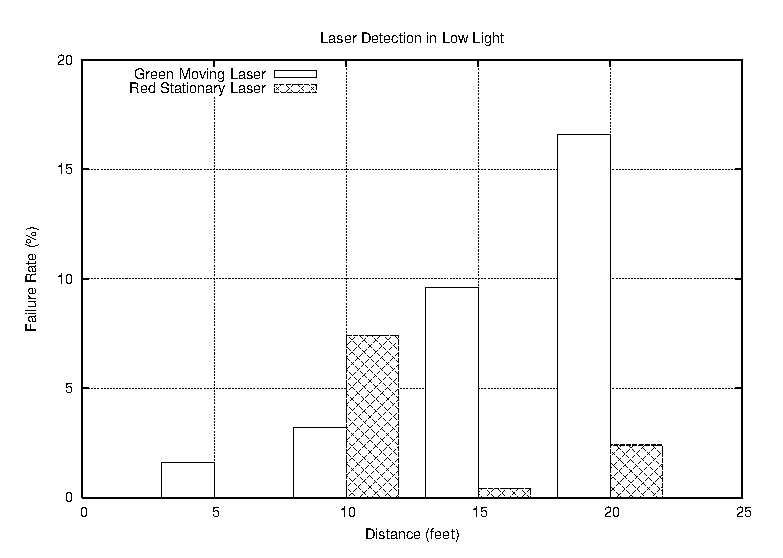
\includegraphics[width=0.8\linewidth]{laser_low.eps}
\end{center}
   \caption{Laser detection in Low Light.}
\label{fig:laser_low}
\label{fig:long}
\label{fig:onecol}
\end{figure}

\begin{figure}[t]
\begin{center}
  \includegraphics[width=0.8\linewidth]{laser_high.eps}
\end{center}
   \caption{Laser detection in High Light.}
\label{fig:laser_high}
\label{fig:long}
\label{fig:onecol}
\end{figure}

\subsection{Distance Estimation}

Figure TODO shows the results of the distance estimation.

The distance estimation was not implemented into the turret aim logic due to the low accuracy at distances over eight feet. One of the problems was that the distance estimation accuracy is directly related to how far the distance laser is mounted away from the optical axis.  

\subsection{Turret Accuracy}


\section{Discussion and Conclusion}


\section{Future Work}
We are using a low cost airsoft gun manufactured b DPMS. It is electrically operated airsoft gun that fires the standard 6mm plastic balls typical of these class of toys. Although many airsoft guns have a muzzle velocity of over 300 feet per second, this particular one is fairly light, rated at only 110 feet per second. The bulk of the turret assembly we be built around effectively mounting this airsoft gun.

We are using a low cost airsoft gun manufactured b DPMS. It is electrically operated airsoft gun that fires the standard 6mm plastic balls typical of these class of toys. Although many airsoft guns have a muzzle velocity of over 300 feet per second, this particular one is fairly light, rated at only 110 feet per second. The bulk of the turret assembly we be built around effectively mounting this airsoft gun.

We are using a low cost airsoft gun manufactured b DPMS. It is electrically operated airsoft gun that fires the standard 6mm plastic balls typical of these class of toys. Although many airsoft guns have a muzzle velocity of over 300 feet per second, this particular one is fairly light, rated at only 110 feet per second. The bulk of the turret assembly we be built around effectively mounting this airsoft gun.


\begin{figure}[t]
\begin{center}
  
\includegraphics[width=0.8\linewidth]{hammer_069_a.eps}
\end{center}
   \caption{Future Revision of our turret.}
\label{fig:long}
\label{fig:onecol}
\end{figure}
We are using a low cost airsoft gun manufactured b DPMS. It is electrically operated airsoft gun that fires the standard 6mm plastic balls typical of these class of toys. Although many airsoft guns have a muzzle velocity of over 300 feet per second, this particular one is fairly light, rated at only 110 feet per second. The bulk of the turret assembly we be built around effectively mounting this airsoft gun.

We are using a low cost airsoft gun manufactured b DPMS. It is electrically operated airsoft gun that fires the standard 6mm plastic balls typical of these class of toys. Although many airsoft guns have a muzzle velocity of over 300 feet per second, this particular one is fairly light, rated at only 110 feet per second. The bulk of the turret assembly we be built around effectively mounting this airsoft gun.

We are using a low cost airsoft gun manufactured b DPMS. It is electrically operated airsoft gun that fires the standard 6mm plastic balls typical of these class of toys. Although many airsoft guns have a muzzle velocity of over 300 feet per second, this particular one is fairly light, rated at only 110 feet per second. The bulk of the turret assembly we be built around effectively mounting this airsoft gun.



\begin{thebibliography}{1}

  \bibitem{olsen01laser} Dan R. Olsen and S. Travis Nielsen {\em Laser pointer interaction.} 2001. 

  \bibitem{nxt} \url{http://www.lego.com/eng/info/default.asp?page=pressdetail&contentid=17278&countrycode=2057&yearcode=&archive=false}

  \bibitem{pynxt} \url{http://home.comcast.net/~dplau/nxt\_python/}
  
	\bibitem{logi} Logitech Website. \url{http://www.logitech.com/index.cfm/webcam\_communications/webcams/devices/352&cl=us,en}

  \bibitem{calpac} Calpac Lasers. \url{http://calpaclasers.com/laser\_pointers.html}


  \end{thebibliography}



\end{document}
